%% Plantilla basada en elsarticle-template-num.tex
%% Formato requerido: elsarticle con referencias numeradas
\documentclass[preprint,12pt]{elsarticle}

\usepackage[utf8]{inputenc}
\usepackage[spanish]{babel}
\usepackage{amssymb}
\usepackage{amsmath,amsfonts}
\usepackage{graphicx}
\usepackage{textcomp}
\usepackage{xcolor}
\usepackage{hyperref}
\usepackage{url}
\usepackage{booktabs}
\usepackage{multirow}
\usepackage{array}

\hypersetup{
    colorlinks=true,
    linkcolor=blue,
    urlcolor=blue,
    citecolor=blue
}

\journal{Estado del Arte -- Proyecto de Deep Learning}

\begin{document}

\begin{frontmatter}

\title{Estado del Arte: Modelos de Deep Learning para la Predicción de Demanda en Transporte Público}

\author{Jose Esteban Otero Rada}

\affiliation{
    organization={Facultad de Ingeniería de Sistemas, Universidad de San Buenaventura Cali},
    addressline={},
    city={Cali},
    postcode={},
    state={Valle del Cauca},
    country={Colombia}
}

\ead{jeoteror@correo.usbcali.edu.co}

\begin{abstract}
Hoy en día la logística del transporte público se basa en horarios fijos o comunicación entre estaciones cuando se presenta una alta demanda, generando inconformidad entre los usuarios por aumentos en los tiempos de espera. Este trabajo presenta un estado del arte sobre el uso de modelos de \textit{deep learning} para predecir la demanda futura de usuarios en una estación o ruta. Se revisan las arquitecturas empleadas en proyectos ya elaborados y se analizan los conjuntos de datos abiertos disponibles. Además, se presenta la metodología experimental del prototipo propuesto y resultados preliminares de predicción horaria de demanda en el metro de Nueva York usando una red BiLSTM, la cual alcanzó un $R^2$ de 0{,}857 en el conjunto de prueba.
\end{abstract}

\end{frontmatter}

%% ---------------------------------------------------------------
\section{Introducción}
%% ---------------------------------------------------------------

El transporte público urbano es uno de los servicios más importantes en una ciudad, ya que su eficiencia impacta directamente en la calidad de vida de los ciudadanos \cite{welch2019}. Sin embargo, la organización de la logística de este servicio ha dependido históricamente de horarios fijos y métodos estadísticos que no logran adaptarse a los cambios en la demanda en tiempo real \cite{afandizadeh2024}. Este enfoque rígido genera estaciones sobrecargadas, tiempos de espera largos e insatisfacción entre los usuarios.

El problema es que la demanda de transporte público no es lineal ni predecible. Variables como la hora del día, las condiciones climáticas, los días festivos, la estacionalidad y eventos sociales alteran el comportamiento de los pasajeros \cite{afandizadeh2024}. Por esta razón, los sistemas de planificación basados en horarios fijos resultan ineficientes. Los sistemas de transporte generan grandes volúmenes de datos históricos de operación que pueden aprovecharse para entrenar modelos capaces de anticipar los patrones de demanda \cite{liyanage2022}.

Este documento tiene como objetivo elaborar un estado del arte que permita identificar qué arquitecturas de \textit{deep learning} se han empleado para este fin, qué fuentes de datos están disponibles públicamente y qué brechas persisten en la literatura. También se presenta la metodología y los resultados del prototipo que se desarrolló. La Sección~2 agrupa todo el estado del arte: la metodología de búsqueda, los trabajos revisados, los vacíos identificados y el dataset seleccionado. La Sección~3 describe los materiales y métodos del prototipo experimental. La Sección~4 presenta los resultados obtenidos. La Sección~5 contiene la discusión e interpretación crítica de los resultados frente a la literatura, y la Sección~6 las conclusiones y trabajo futuro.


%% ---------------------------------------------------------------
\section{Estado del Arte}
%% ---------------------------------------------------------------

\subsection{Metodología de Búsqueda Bibliográfica}

Para identificar los trabajos más relevantes y actuales, se definió una búsqueda acotada entre los años 2020 y 2024, con el fin de obtener información sobre el estado actual de las técnicas de \textit{deep learning} aplicadas al transporte. En paralelo, se revisaron portales de datos abiertos de agencias de transporte, priorizando aquellos que ofrecen registros históricos con granularidad horaria. Se incluyeron trabajos que cumplieran al menos uno de estos criterios: artículos de revisión sistemática sobre \textit{deep learning} en transporte público, estudios experimentales en repositorios académicos de acceso abierto, y documentación técnica oficial de estándares de datos de transporte.

\subsection{De los Modelos Clásicos al Deep Learning}

La predicción de la demanda en transporte público no es un problema nuevo. Los modelos estadísticos tradicionales como ARIMA y el Filtro de Kalman fue lo que se usó para esta situación, pero estos modelos presentan limitaciones cuando se aplican a entornos reales.

Afandizadeh et al.\ \cite{afandizadeh2024} presentan una revisión en la que demuestran que los modelos clásicos son robustos para series de tiempo estables y con comportamiento lineal, pero fallan en escenarios de tráfico caótico donde intervienen múltiples variables. Su estudio concluye que las redes neuronales profundas superan estas limitaciones al capturar la no linealidad del tráfico urbano, integrando además variables externas como las condiciones climáticas.

\subsection{Redes LSTM y BiLSTM para Series Temporales de Transporte}

Xu y Jin \cite{xu2021} proponen un modelo basado en LSTM para la predicción del flujo de pasajeros a corto plazo en buses urbanos, y concluyen que la principal ventaja de esta arquitectura está en su capacidad de retener dependencias a largo plazo en la secuencia temporal. Esto resulta importante en el contexto del transporte, donde los patrones de demanda presentan periodicidades claras a nivel diario y semanal.

Utku y Kaya \cite{utku2023} desarrollaron un modelo LSTM multicapa para predecir el flujo de pasajeros a corto plazo en las rutas de transporte de Estambul, utilizando datos del año 2020 con intervalos de una hora. El modelo fue comparado con otras arquitecturas mostrando que la LSTM ofrece el mejor desempeño cuando se trabaja con series horarias largas. En la línea de las redes bidireccionales, Ma et al.\ \cite{ma2018} propusieron una arquitectura paralela de CNN y BiLSTM para la predicción de la demanda en toda la red del metro de Beijing, demostrando que la combinación bidireccional captura mejor las correlaciones espacio-temporales que las arquitecturas unidireccionales.

\subsection{Procesamiento de Smart Card Data}

Una de las fuentes de datos para el entrenamiento de estos modelos son los registros de tarjetas inteligentes de acceso al transporte público. Pelletier et al.\ \cite{pelletier2011} realizan una revisión de literatura sobre el uso de datos de tarjetas inteligentes en transporte público dónde señalan que los datos de tarjetas inteligentes ofrecen atributos únicos como identificador de usuario, ubicación exacta del punto de abordaje y marca de tiempo precisa, pero requieren un preprocesamiento riguroso como la normalización de los valores numéricos y la agregación temporal en ventanas de 15, 30 o 60 minutos.

\subsection{El Estándar GTFS como Infraestructura de Datos}

El estándar GTFS (\textit{General Transit Feed Specification}) \cite{gtfs_home} es la base para describir la información de los sistemas de transporte público. El estándar permite representar rutas, paradas, viajes y calendarios de servicio en archivos de texto estructurados \cite{gtfs_using, gtfs_sharing}. Para garantizar la calidad de los feeds publicados, la comunidad ha definido buenas prácticas de estructura y documentación \cite{gtfs_bestpractices, tumi_gtfs}. Un ejemplo concreto de adopción es la agencia AC Transit del Área de la Bahía de San Francisco, que publica su feed GTFS de forma abierta y actualizada \cite{actransit_gtfs}.

\subsection{Modelos Basados en Grafos para Múltiples Estaciones}

Los modelos LSTM y BiLSTM funcionan bien con una sola estación, pero cuando se quiere predecir la demanda de varias estaciones a la vez se necesita representar cómo se relacionan entre sí. Para eso sirven las redes de grafos o GNN (\textit{Graph Neural Networks}), que tratan las estaciones como nodos y las conexiones entre ellas como aristas.

Yu et al.\ \cite{yu2018} propusieron un modelo que combina convoluciones sobre grafos con convoluciones temporales, obteniendo mejores resultados que los modelos LSTM de ese momento. Jiang y Deng \cite{jiang2022} revisaron trabajos entre 2020 y 2024 y encontraron que más de la mitad ya usaban algún tipo de GCN para manejar la parte espacial del problema. Wang y Shalaby \cite{wang2024} presentaron DST-TransitNet, que combina GNN con GRU y mecanismos de atención, logrando reducir el RMSE entre un 8\% y 15\% frente a LSTM en datos del metro de Toronto gracias a pesos espaciales dinámicos.

La ventaja de estos modelos es que capturan cómo la demanda de una estación afecta a las vecinas, aunque son más complejos de implementar y demandan más recursos computacionales.

\subsection{Arquitecturas Basadas en Mecanismos de Atención y Transformers}

Bapaume et al.\ \cite{bapaume2023} usaron un Transformer para predecir el flujo de pasajeros en la línea 9 del metro de París, planteando el problema como la completación de una imagen bidimensional de demanda por estación y hora. El modelo mostró robustez ante eventos disruptivos como huelgas. He et al.\ \cite{he2024} propusieron un módulo híbrido que integra capas Transformer con GRU prescindiendo de la estructura de grafo explícita, obteniendo precisiones competitivas con menor complejidad de ingeniería. Este hallazgo sugiere que es posible alcanzar resultados similares a los modelos de grafos sin la carga que implica construir y mantener la estructura de adyacencia.

\subsection{Métricas de Evaluación en la Predicción de Demanda}

Los trabajos revisados emplean un conjunto común de métricas para evaluar el rendimiento de los modelos. El MAE (\textit{Mean Absolute Error}) mide el error absoluto promedio en unidades de pasajeros. El RMSE (\textit{Root Mean Squared Error}) es la métrica dominante en la mayoría de los estudios, ya que penaliza con más fuerza los errores grandes. El MAPE (\textit{Mean Absolute Percentage Error}) expresa el error como porcentaje del valor real, lo que facilita comparar estaciones con distintos niveles de demanda. El $R^2$ o coeficiente de determinación indica qué proporción de la variabilidad de los datos reales logra explicar el modelo. Un problema identificado es que no todos los trabajos reportan las mismas métricas, lo que dificulta la comparación directa entre estudios.

\subsection{Vacíos Identificados}

La revisión identificó tres áreas donde hay espacio para aportar desde proyectos académicos.

Interpretabilidad de los modelos: la mayoría de las arquitecturas revisadas actúan como cajas negras que producen predicciones con alta precisión, pero no ofrecen una explicación de los factores que determinan ese resultado. Esta limitación dificulta su adopción en entornos operativos donde los tomadores de decisiones requieren justificaciones claras.

Escasez de datos abiertos estandarizados: aunque existen repositorios de datos públicos, son pocos los conjuntos de datos documentados y estructurados que permitan comparar algoritmos de forma reproducible en distintas ciudades. La mayoría de los estudios revisados trabajan con datos propietarios o con conjuntos específicos de una sola ciudad, lo que limita la generalización de los resultados.

Eficiencia computacional: la mayoría de los modelos de alto rendimiento reportados en la literatura requieren infraestructuras de cómputo significativas tanto para el entrenamiento como para la inferencia. Esto representa una barrera para su despliegue en sistemas de ciudades medianas con recursos tecnológicos limitados.

\subsection{Análisis Comparativo de Trabajos Revisados}

La Tabla~\ref{tab:comparativo} presenta una comparativa de los principales trabajos revisados, organizada por arquitectura empleada, fuente de datos, métricas reportadas y hallazgo principal.

\begin{table}[htbp]
\centering
\caption{Comparación de trabajos revisados sobre predicción de demanda en transporte público.}
\label{tab:comparativo}
\small
\begin{tabular}{p{2.2cm} p{2cm} p{2.2cm} p{1.5cm} p{3.8cm}}
\toprule
\textbf{Referencia} & \textbf{Arquitectura} & \textbf{Datos} & \textbf{Métricas} & \textbf{Hallazgo principal} \\
\midrule
Afandizadeh et al.\ \cite{afandizadeh2024} & Revisión (DL vs.\ clásicos) & Múltiples & --- & DL supera a modelos clásicos en escenarios no lineales \\
\addlinespace
Xu y Jin \cite{xu2021} & LSTM & Buses (China) & RMSE, MAE & LSTM captura dependencias a largo plazo en demanda de bus \\
\addlinespace
Utku y Kaya \cite{utku2023} & LSTM multicapa & Transit Estambul & MAE, RMSE, $R^2$ & LSTM supera RF, SVM, ARIMA, MLP y CNN en series horarias \\
\addlinespace
Mamede et al.\ \cite{mamede2023} & LSTM vs.\ ARIMA & Centros de distribución (Brasil) & RMSE, MAE & LSTM supera ARIMA en 94\% de los escenarios \\
\addlinespace
Liyanage et al.\ \cite{liyanage2022} & BiLSTM & Smart Card (Melbourne) & RMSE, $R^2$ & BiLSTM supera a LSTM con precisión $>$90\% (15--30 min) \\
\addlinespace
Ma et al.\ \cite{ma2018} & CNN + BiLSTM paralela & Metro Beijing & RMSE, MAE & Arquitectura paralela captura correlaciones espacio-temporales \\
\addlinespace
Yu et al.\ \cite{yu2018} & STGCN & Tráfico vehicular & MAE, MAPE & Convolución de grafos + temporal supera a LSTM en redes \\
\addlinespace
Wang y Shalaby \cite{wang2024} & GNN+GAT+GRU & Metro y buses (Toronto) & RMSE, MAE & Pesos espaciales dinámicos reducen RMSE 8--15\% vs.\ LSTM \\
\addlinespace
He et al.\ \cite{he2024} & DT-GRU & Metro (China) & RMSE, MAE, MAPE & Alcanza nivel GCN sin estructura de grafo explícita \\
\addlinespace
Bapaume et al.\ \cite{bapaume2023} & Transformer & Metro línea 9 (París) & MAE, RMSE & Robusto ante eventos atípicos (huelgas) \\
\addlinespace
\bottomrule
\end{tabular}
\end{table}

Del análisis comparativo se extraen tres observaciones clave para este proyecto. Primero, las arquitecturas espacio-temporales ofrecen el mejor rendimiento cuando se dispone de una red con múltiples estaciones interconectadas. Segundo, los modelos híbridos que combinan preprocesamiento cuidadoso con arquitecturas recurrentes logran resultados competitivos con menor complejidad. Tercero, un buen diseño del pipeline de datos puede ser más determinante que la búsqueda de arquitecturas más complejas. 

\subsection{Dataset Seleccionado}

Tras revisar varios repositorios de datos públicos, se determinó que el portal de datos abiertos del estado de Nueva York (\texttt{data.ny.gov}) ofrece la colección más adecuada para los objetivos del proyecto. El dataset principal es el MTA Subway Hourly Ridership (2025) \cite{mta_hourly}, que proporciona estimaciones de la demanda de pasajeros en franjas horarias, desglosadas por estación y por método de pago. El dataset ya viene filtrado por modo subway y categoría tarifaria Full Fare, y cuenta con 6.570.508 filas y 12 columnas, bajo la licencia NYC Open Data Terms of Use que permite su uso académico libre.



%% ---------------------------------------------------------------
\section{Materiales y Métodos}
%% ---------------------------------------------------------------

En esta sección se detalla la selección y justificación del dataset, las variables externas incorporadas, el preprocesamiento aplicado, ejemplos de las series temporales construidas, la arquitectura del modelo y el protocolo de entrenamiento y evaluación.

\subsection{Selección y Justificación del Dataset}

Se seleccionó el MTA Subway Hourly Ridership (2025) \cite{mta_hourly} como fuente del proyecto, por tres razones principales. La granularidad horaria permite entrenar modelos de series temporales. \cite{liyanage2022, ghandeharioun2023}. La inclusión de coordenadas geográficas. Y los datos del sistema MTA de Nueva York han sido empleados en trabajos previos \cite{ghandeharioun2023, wang2024}, lo que facilita la comparación cuantitativa de resultados.

El dataset contiene las columnas: \texttt{transit\_timestamp}, \texttt{transit\_mode}, \texttt{station\_complex\_id} (identificador alfanumérico del complejo de estaciones), \texttt{station\_complex}, \texttt{borough} (5 distritos: Manhattan, Brooklyn, Queens, Bronx y Staten Island), \texttt{payment\_method} (MetroCard u OMNY), \texttt{fare\_class\_category}, \texttt{ridership}, \texttt{transfers}, \texttt{latitude}, \texttt{longitude} y \texttt{Georeference}.

\subsection{Enriquecimiento con Variables Externas}

Incorporar variables climáticas y temporales como covariables de entrenamiento mejoría la capacidad predictiva de los modelos \cite{afandizadeh2024, liu2024}. El dataset primario se enriquece con dos fuentes externas.

Datos climáticos: se obtienen datos meteorológicos históricos horarios para las coordenadas de Nueva York durante 2025. Las variables seleccionadas son temperatura, precipitación, humedad relativa, velocidad del viento y código de condición climática WMO.

Calendario de festivos: se construye una variable binaria \texttt{is\_holiday} que toma el valor 1 en los días festivos federales y estatales de Nueva York en 2025 \cite{nyc_holidays_2025} y 0 en los demás días. 
\subsection{Muestra de la Serie Temporal}

Para ilustrar cómo se ven los datos en la práctica, la Tabla~\ref{tab:muestra} presenta 10 registros correspondientes al 8 de enero de 2025.

\begin{table}[htbp]
\centering
\caption{Muestra de 10 registros del dataset integrado — Estación Astoria-Ditmars Blvd (N,W), 8 de enero de 2025.}
\label{tab:muestra}
\small
\begin{tabular}{cccccccc}
\toprule
\textbf{Hora} & \textbf{Ridership} & \textbf{Temp.} & \textbf{Precip.} & \textbf{Hum.} & \textbf{Viento} & \textbf{Festivo} & \textbf{Fin sem.} \\
 & \textbf{(pasaj.)} & \textbf{(°C)} & \textbf{(mm)} & \textbf{(\%)} & \textbf{(km/h)} & & \\
\midrule
01:00 & 11  & -4,0 & 0,0 & 55 & 17,0 & 0 & 0 \\
02:00 & 5   & -4,0 & 0,0 & 55 & 20,2 & 0 & 0 \\
03:00 & 13  & -4,1 & 0,0 & 55 & 19,9 & 0 & 0 \\
04:00 & 34  & -4,3 & 0,0 & 55 & 20,2 & 0 & 0 \\
05:00 & 158 & -4,4 & 0,0 & 56 & 18,6 & 0 & 0 \\
06:00 & 486 & -4,3 & 0,0 & 57 & 16,5 & 0 & 0 \\
07:00 & 983 & -4,4 & 0,0 & 57 & 17,5 & 0 & 0 \\
08:00 & 182 & -4,8 & 0,0 & 58 & 15,8 & 0 & 0 \\
09:00 & 824 & -4,1 & 0,0 & 50 & 17,3 & 0 & 0 \\
10:00 & 418 & -3,5 & 0,0 & 45 & 18,5 & 0 & 0 \\
\bottomrule
\end{tabular}
\end{table}

Para entrenar la red neuronal, estos registros se transforman en ventanas deslizantes. La Tabla~\ref{tab:ventana} ilustra de forma simplificada cómo se construye una muestra de entrenamiento: se toman $T = 48$ horas consecutivas de entrada (cada fila es un vector de todas las variables de la Tabla~\ref{tab:dataset_final}) y el modelo debe predecir el valor de \texttt{ridership} en la hora $T+1$.

\subsection{Descripción del Dataset Resultante}

Tras la fusión y el enriquecimiento, el dataset final contiene un registro por cada combinación de estación y hora durante el año 2025. La Tabla~\ref{tab:dataset_final} resume las características del dataset resultante.

Mostrando los datos cualitativos y cuantitativos del dataset y los las variables que lo conforman.

\begin{table}[htbp]
\centering
\caption{Características del dataset integrado para entrenamiento.}
\label{tab:dataset_final}
\small
\begin{tabular}{p{4cm} p{8.5cm}}
\toprule
\textbf{Atributo} & \textbf{Descripción} \\
\midrule
Tamaño & 6.570.508 filas × 12 columnas \\
Cobertura temporal & 1 de enero -- 31 de diciembre de 2025 \\
Resolución temporal & 1 hora \\
Modo de transporte & Subway (metro) \\
Categoría tarifaria & Full Fare (MetroCard + OMNY) \\
N.º de estaciones & $\approx$472 complejos de estaciones \\
N.º de distritos & 5 (Manhattan, Brooklyn, Queens, Bronx, Staten Island) \\
Licencia (dataset MTA) & NYC Open Data Terms of Use \\
Licencia (datos clima) & CC BY 4.0 (Open-Meteo / ERA5) \\
\midrule
\multicolumn{2}{l}{\textit{Variables del dataset primario}} \\
\midrule
\texttt{transit\_timestamp} & Marca temporal (hora) \\
\texttt{station\_complex\_id} & Identificador del complejo de estaciones \\
\texttt{borough} & Distrito \\
\texttt{ridership} & Número de pasajeros (variable objetivo) \\
\texttt{latitude}, \texttt{longitude} & Coordenadas geográficas \\
\midrule
\multicolumn{2}{l}{\textit{Variables derivadas}} \\
\midrule
\texttt{hour\_sin}, \texttt{hour\_cos} & Hora del día codificada en forma cíclica \\
\texttt{dow\_sin}, \texttt{dow\_cos} & Día de la semana codificado en forma cíclica \\
\texttt{month\_sin}, \texttt{month\_cos} & Mes del año codificado en forma cíclica \\
\texttt{is\_weekend} & Indicador binario de fin de semana \\
\texttt{ridership\_lag\_24h} & Demanda de la misma estación hace 24 horas \\
\texttt{ridership\_lag\_168h} & Demanda de la misma estación hace 168 horas (1 semana) \\
\midrule
\multicolumn{2}{l}{\textit{Variables externas (clima y festivos)}} \\
\midrule
\texttt{temperature\_2m} & Temperatura (°C) \\
\texttt{precipitation} & Precipitación acumulada en la hora (mm) \\
\texttt{relative\_humidity\_2m} & Humedad relativa (\%) \\
\texttt{wind\_speed\_10m} & Velocidad del viento (km/h) \\
\texttt{is\_holiday} & Indicador binario de día festivo \\
\bottomrule
\end{tabular}
\end{table}



\begin{table}[htbp]
\centering
\caption{Ejemplo simplificado de ventana deslizante ($T = 4$, $h = 1$) para la construcción de una muestra de entrenamiento.}
\label{tab:ventana}
\small
\begin{tabular}{ccccc}
\toprule
\textbf{Paso} & \textbf{Hora} & \textbf{Ridership} & \textbf{Temp. (°C)} & \textbf{Rol en el modelo} \\
\midrule
$t-3$ & 01:00 & 11  & -4,0 & \multirow{4}{*}{Entrada (contexto)} \\
$t-2$ & 02:00 & 5   & -4,0 & \\
$t-1$ & 03:00 & 13  & -4,1 & \\
$t$   & 04:00 & 34  & -4,3 & \\
\midrule
$t+1$ & 05:00 & 158 & -4,4 & Etiqueta (valor a predecir) \\
\bottomrule
\end{tabular}
\end{table}


\subsection{Preprocesamiento de Datos}

El pipeline de preprocesamiento consta de las siguientes etapas:

1. Limpieza: se eliminan registros con valores nulos en \texttt{ridership} o \texttt{transit\_timestamp}. 

2. Conversión temporal: la columna \texttt{transit\_timestamp} se convierte a formato \texttt{datetime}.

3. Agregación por método de pago: se agrupa por \texttt{transit\_timestamp} y \texttt{station\_complex\_id}, sumando el \texttt{ridership} de MetroCard y OMNY para obtener el total de pasajeros por estación y hora.

4. Fusión con datos climáticos: se realiza un \textit{merge} entre el dataset y los datos de Open-Meteo usando la fecha y hora como clave, con tolerancia de 1 hora.

5. Incorporación de festivos: se añade la columna \texttt{is\_holiday} mediante un \textit{merge} por fecha con el calendario de festivos de NYC 2025.

6. Normalización: las variables numéricas se escalan usando z-score por estación (se resta la media y se divide por la desviación estándar de cada estación). Las variables periódicas (hora, día de la semana, mes) se codifican mediante seno y coseno para evitar discontinuidades en sus límites. Los parámetros de normalización se calculan exclusivamente con los datos de entrenamiento para evitar fuga de información al conjunto de prueba.

7. Construcción de ventanas deslizantes: se construyen secuencias de entrada de longitud $T = 48$ horas y se asigna como etiqueta el valor de \texttt{ridership} en el paso $T+1$.

8. Partición temporal: los datos se dividen cronológicamente en entrenamiento (70\%, enero--septiembre), validación (15\%, octubre--mediados de noviembre) y prueba (15\%, mediados de noviembre--diciembre).

\subsection{Arquitectura del Modelo Propuesto}

Tomando como base los resultados de Liyanage et al.\ \cite{liyanage2022} sobre la superioridad de la BiLSTM frente a la LSTM unidireccional, y de Ghandeharioun et al.\ \cite{ghandeharioun2023} sobre la importancia de la granularidad temporal frente a la complejidad arquitectónica, se propone una arquitectura con las siguientes capas:

Capa de entrada: recibe secuencias de forma $(T, F)$, donde $T$ es la longitud de la ventana y $F$ el número de variables.

Capa BiLSTM 1: 64 unidades, con \texttt{return\_sequences=True} para el apilamiento de capas. Se aplica Dropout con tasa de 0,2 para regularización.

Capa BiLSTM 2: 32 unidades, con \texttt{return\_sequences=False}. Se aplica Dropout con tasa de 0,2.

Capa densa intermedia: 32 neuronas con función de activación ReLU.

Capa de salida: 1 neurona con activación lineal, que produce la predicción del \texttt{ridership} normalizado para la hora siguiente.

La Figura~\ref{fig:arquitectura} ilustra la arquitectura de forma esquemática.

\begin{figure}[htbp]
\centering
\fbox{\parbox{0.9\textwidth}{\centering
\small
\texttt{Entrada $(T, F)$} $\longrightarrow$
\texttt{BiLSTM-64} $\longrightarrow$
\texttt{Dropout(0.2)} $\longrightarrow$
\texttt{BiLSTM-32} $\longrightarrow$
\texttt{Dropout(0.2)} $\longrightarrow$
\texttt{Dense-32 (ReLU)} $\longrightarrow$
\texttt{Dense-1 (Lineal)}
}}
\caption{Arquitectura del modelo BiLSTM propuesto para la predicción de demanda horaria.}
\label{fig:arquitectura}
\end{figure}

La Tabla~\ref{tab:hiperparametros} resume los hiperparámetros del modelo.

\begin{table}[htbp]
\centering
\caption{Hiperparámetros del modelo propuesto.}
\label{tab:hiperparametros}
\small
\begin{tabular}{p{4.5cm} p{3cm} p{4.5cm}}
\toprule
\textbf{Hiperparámetro} & \textbf{Valor inicial} & \textbf{Rango de exploración} \\
\midrule
Unidades BiLSTM capa 1 & 64 & \{64, 128, 256\} \\
Unidades BiLSTM capa 2 & 32 & \{32, 64, 128\} \\
Tasa de Dropout & 0,2 & \{0,1, 0,2, 0,3\} \\
Neuronas capa densa & 32 & \{16, 32, 64\} \\
Ventana temporal ($T$) & 48 horas & \{12, 24, 48\} \\
Horizonte de predicción ($h$) & 1 hora & \{1, 6, 24\} \\
Tasa de aprendizaje & 0,001 & \{0,0001, 0,001, 0,01\} \\
Tamaño de batch & 64 & \{32, 64, 128\} \\
Épocas máximas & 100 & --- \\
\bottomrule
\end{tabular}
\end{table}

\subsection{Protocolo de Entrenamiento}

El entrenamiento se realizó en TensorFlow/Keras con los siguientes componentes. Como función de pérdida se usó el error cuadrático medio (MSE), compatible con el RMSE empleado en la evaluación. Como optimizador se usó Adam con tasa de aprendizaje inicial de 0,001 y un planificador ReduceLROnPlateau que reduce la tasa en un factor de 0,5 cuando la pérdida de validación no mejora durante 5 épocas consecutivas. Se activó Early Stopping con \texttt{patience=10}, restaurando los pesos de la mejor época registrada. El entorno de ejecución fue Google Colab con GPU T4.

\subsection{Protocolo de Evaluación}

El rendimiento del modelo se evaluó en el conjunto de prueba usando las cuatro métricas identificadas en la revisión de literatura (Sección~2.8):

\begin{itemize}
    \item MAE (\textit{Mean Absolute Error}): $\text{MAE} = \frac{1}{n} \sum_{i=1}^{n} |y_i - \hat{y}_i|$
    \item RMSE (\textit{Root Mean Squared Error}): $\text{RMSE} = \sqrt{\frac{1}{n} \sum_{i=1}^{n} (y_i - \hat{y}_i)^2}$
    \item MAPE (\textit{Mean Absolute Percentage Error}): $\text{MAPE} = \frac{100}{n} \sum_{i=1}^{n} \left|\frac{y_i - \hat{y}_i}{y_i}\right|$
    \item $R^2$ (Coeficiente de determinación): $R^2 = 1 - \frac{\sum_{i=1}^{n}(y_i - \hat{y}_i)^2}{\sum_{i=1}^{n}(y_i - \bar{y})^2}$
\end{itemize}

donde $y_i$ es el valor real, $\hat{y}_i$ es el valor predicho, $\bar{y}$ es la media de los valores reales y $n$ es el número de observaciones en el conjunto de prueba.

Adicionalmente, se realizaron dos análisis complementarios. El primero es la comparación con líneas base: un modelo LSTM unidireccional con la misma configuración y un modelo naive que predice que el valor futuro será igual al de la misma hora del día anterior. El segundo es el análisis de ablación, donde se entrenó el modelo con y sin las variables climáticas para cuantificar su contribución al rendimiento.


%% ---------------------------------------------------------------
\section{Resultados}
%% ---------------------------------------------------------------

Esta sección presenta los resultados obtenidos al ejecutar el pipeline experimental descrito en la Sección~3. Se reportan tanto los resultados cuantitativos como cualitativos sobre una estación piloto representativa del sistema de metro de Nueva York.

\subsection{Configuración Experimental}

Tras el preprocesamiento y la limpieza de datos, el dataset resultante conservó 399 estaciones de las 472 originales, eliminando aquellas con menos de 8.000 registros horarios. Como estación piloto se seleccionó 110 St--Malcolm X Plaza, correspondiente a la estación de demanda mediana del ranking, con una demanda promedio horaria de 137 pasajeros y 8.520 registros válidos. La elección de una estación de demanda media, en lugar de la de mayor volumen, permite evaluar el rendimiento del modelo en un escenario representativo del sistema, evitando sesgos hacia estaciones de alto tráfico. El entrenamiento se detuvo en la época 29 por efecto del Early Stopping.

\subsection{Resultados Cuantitativos}

La Tabla~\ref{tab:resultados} presenta las métricas de evaluación en el conjunto de prueba para los cuatro modelos evaluados.

\begin{table}[htbp]
\centering
\caption{Métricas de evaluación en el conjunto de prueba — Estación 110 St--Malcolm X Plaza.}
\label{tab:resultados}
\small
\begin{tabular}{lcccc}
\toprule
\textbf{Modelo} & \textbf{MAE} & \textbf{RMSE} & \textbf{MAPE (\%)} & \textbf{$R^2$} \\
\midrule
Naive (lag 24h)       & 34,25 & 58,75 & 32,33 & 0,768 \\
LSTM unidireccional   & 32,12 & 46,46 & 51,32 & 0,855 \\
BiLSTM sin clima      & 30,38 & 46,14 & 43,02 & 0,857 \\
BiLSTM con clima      & 31,71 & 47,17 & 38,17 & 0,850 \\
\bottomrule
\end{tabular}
\end{table}

Los tres modelos de \textit{deep learning} superan al modelo naive en MAE y RMSE, lo que confirma que las redes recurrentes capturan patrones temporales que la persistencia diaria no puede reproducir. Esto se debe a que el naive no puede anticipar variaciones día a día: si el lunes hubo más demanda que el martes anterior, el naive simplemente replicará el martes anterior sin ajustarse.

El BiLSTM sin clima obtiene el mejor rendimiento global y un $R^2$ de 0,857, lo que indica que el modelo explica el 85,7\% de la varianza de la demanda real. La comparación entre LSTM y BiLSTM sin clima muestra que el procesamiento bidireccional aporta una mejora real aunque moderada: el MAE baja de 32,12 a 30,38 (5,4\%) y el RMSE de 46,46 a 46,14. Esto es coherente con los hallazgos de Liyanage et al.\ \cite{liyanage2022}, quienes también reportan que la BiLSTM captura contextos que la LSTM unidireccional no detecta, aunque la magnitud de la ganancia depende del dataset.

El resultado más inesperado es que agregar las variables climáticas no mejora el rendimiento: el BiLSTM con clima tiene un MAE de 31,71 frente a 30,38 del modelo sin clima. Esto puede ser porque la estación piloto es subterránea, donde los pasajeros no están expuestos directamente al clima, lo que reduce la sensibilidad de la demanda a factores meteorológicos. Sin embargo, el modelo con clima obtiene el MAPE más bajo de todos (38,17\%), lo que indica que comete errores relativamente menores en las horas de baja demanda. Esto sugiere que el clima sí aporta información en franjas horarias donde los patrones temporales puros son menos predecibles, como la madrugada o las horas intermedias.
\subsection{Resultados Cualitativos}

\subsubsection{Curvas de Entrenamiento}

La Figura~\ref{fig:curvas} muestra la evolución de la pérdida (MSE) y del MAE durante las 29 épocas. Se observa una convergencia rápida en las primeras 5 épocas. A partir de la época 10, la pérdida de validación se estabiliza mientras la de entrenamiento continúa descendiendo, lo que indica un sobreajuste moderado. La brecha entre ambas curvas es controlada gracias al Dropout y al Early Stopping, que detiene el entrenamiento antes de que el sobreajuste se agrave. En iteraciones futuras podría explorarse una tasa de Dropout mayor para reducir aún más esta brecha.

\begin{figure}[htbp]
\centering
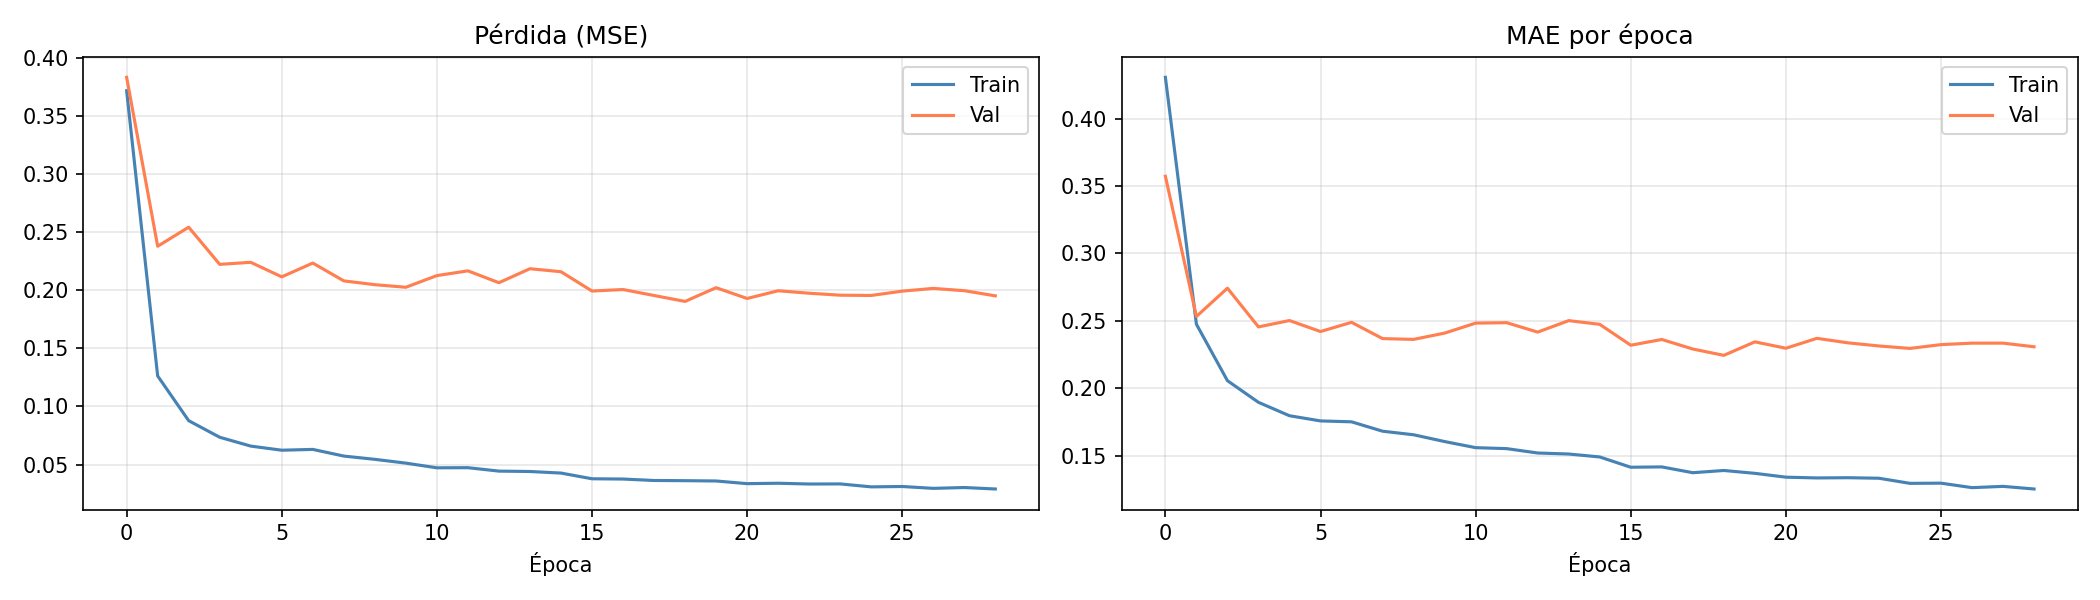
\includegraphics[width=\textwidth]{curvas_entrenamiento.png}
\caption{Evolución de la pérdida (MSE) y el MAE durante el entrenamiento del modelo BiLSTM con clima. La brecha train-val indica sobreajuste moderado controlado por Early Stopping.}
\label{fig:curvas}
\end{figure}


\subsubsection{Análisis de Residuos}

La Figura~\ref{fig:residuos} muestra el diagrama de dispersión real vs.\ predicho y el histograma de residuos del modelo BiLSTM con clima. En el diagrama de dispersión se puede ver que la mayoría de los puntos se concentran cerca de la línea de predicción perfecta, lo que confirma el buen ajuste general indicado por el $R^2 = 0{,}850$. Pero, a medida que la demanda real supera los 300 pasajeros por hora y el modelo predice valores más bajos de los que ocurren en realidad.

El histograma de residuos muestra una distribución centrada ligeramente a la derecha de cero, con una cola más pronunciada hacia valores negativos. Esto indica que aunque el modelo acierta en la mayoría de los casos, en determinadas horas predice más pasajeros de los que realmente llegaron, lo que puede asociarse a eventos que redujeron la demanda de forma inesperada y que las variables de entrada no capturan.

\begin{figure}[htbp]
\centering
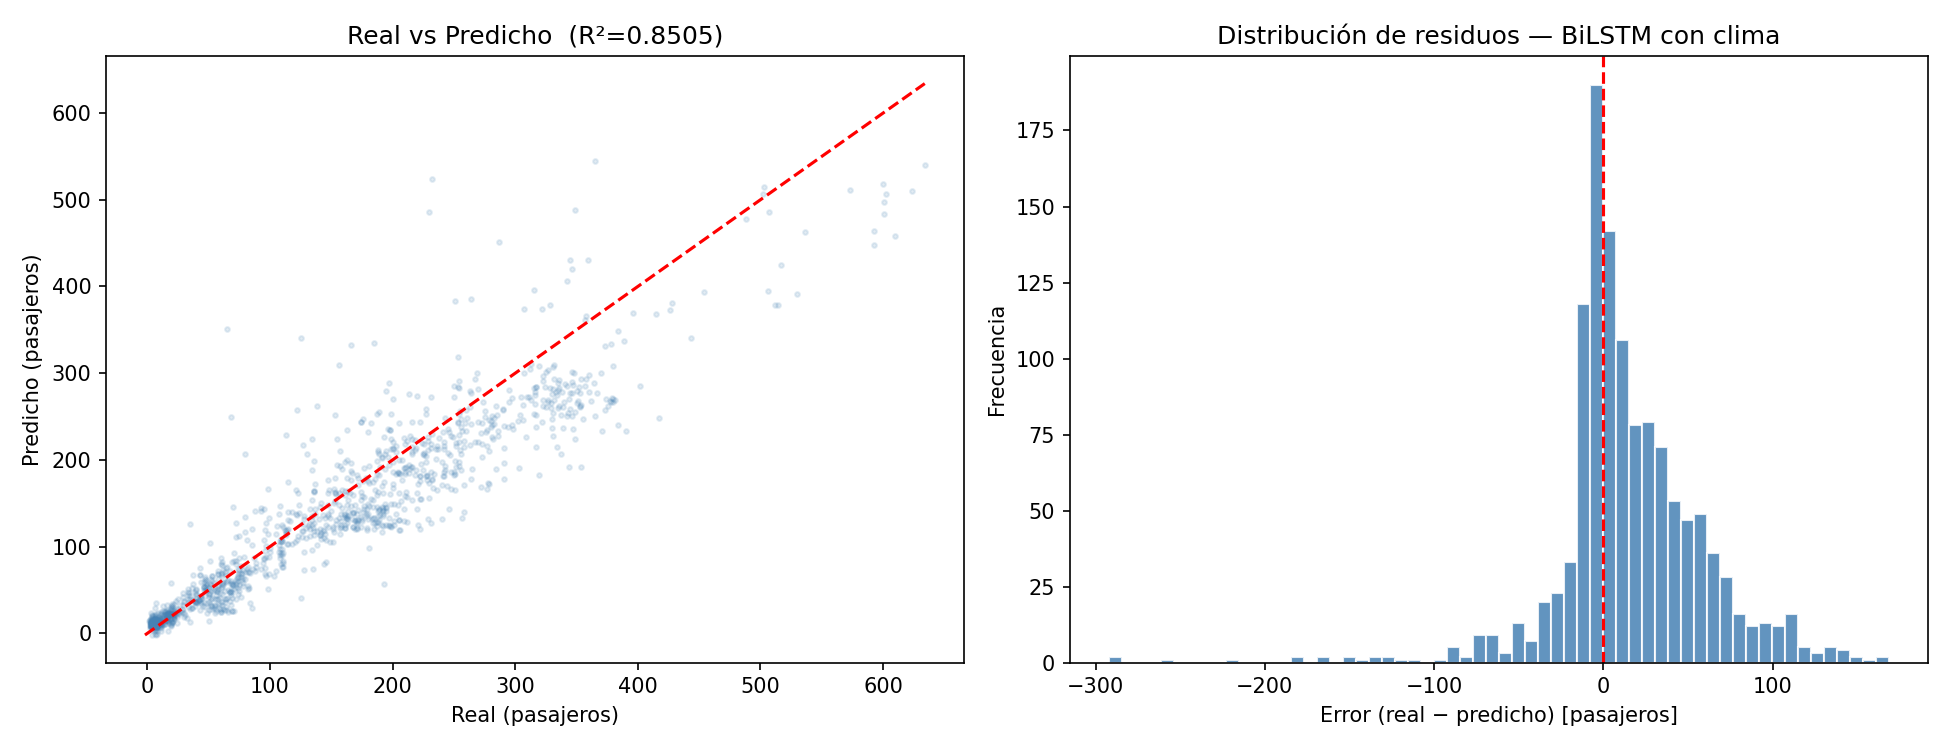
\includegraphics[width=\textwidth]{residuos.png}
\caption{Diagrama real vs.\ predicho ($R^2 = 0{,}850$) y distribución de residuos del modelo BiLSTM con clima.}
\label{fig:residuos}
\end{figure}


%% ---------------------------------------------------------------
\section{Discusión}
%% ---------------------------------------------------------------

Esta sección interpreta los resultados obtenidos en el contexto del problema de predicción de demanda en transporte público y los compara con los hallazgos reportados en el estado del arte.

\subsection{Comparación con la Literatura}

El $R^2$ de 0,857 obtenido por el modelo BiLSTM es consistente con los rangos reportados en la literatura para predicciones horarias en estaciones individuales. Liyanage et al.\ \cite{liyanage2022} reportan precisiones superiores al 90\% en BiLSTM aplicada a Smart Card Data de Melbourne, aunque trabajan con horizontes de 15 a 30 minutos en lugar de una hora, lo que naturalmente facilita la predicción al reducir la incertidumbre del intervalo. La ganancia del 5,4\% en MAE del modelo BiLSTM respecto a LSTM unidireccional está alineada con los resultados de Liyanage et al.\ \cite{liyanage2022} y Ma et al.\ \cite{ma2018}, quienes también reportan mejoras moderadas pero consistentes al pasar a procesamiento bidireccional. 

\subsection{Interpretación del Resultado de la Ablación Climática}

El resultado de la integrar variables climáticas es interesante, mientras que Afandizadeh et al.\ \cite{afandizadeh2024} y Radfar et al.\ \cite{radfar2025} reportaron mejoras al incorporar variables meteorológicas en modelos de demanda de bus en superficie, en este caso la incorporación de clima no mejoró el rendimiento global sino que lo redujo ligeramente. La posible explicación puede se que la estación piloto es una estación subterránea del metro, donde los pasajeros no están expuestos directamente al clima mientras esperan. Esto contrasta con sistemas de bus o paradas de tren ligero al aire libre, donde la decisión de tomar el transporte puede verse fuertemente afectada por lluvia, frío extremo o calor.

\subsection{Limitaciones del Estudio}

Una de las limitaciones de esta revisión es que los resultados corresponden a una sola estación piloto y no se ha validado que las conclusiones se generalicen a estaciones de alto o bajo tráfico, ni a estaciones de superficie donde el comportamiento del clima podría cambiar. 

\subsection{Aporte Original del Trabajo}

Pese a las limitaciones anteriores, este trabajo aporta tres elementos originales al conjunto de evidencia existente. Primero, presenta una comparación cuantitativa controlada entre cuatro modelos (naive, LSTM, BiLSTM sin clima, BiLSTM con clima) sobre la misma estación, lo que permite aislar el aporte del procesamiento bidireccional y del enriquecimiento climático. Segundo, identifica que en estaciones subterráneas el clima no aporta a la métrica global pero sí mejora el error relativo en horas de baja demanda, observación que no aparece en los trabajos revisados. Tercero, todo el pipeline se ejecuta en un entorno gratuito (Google Colab con GPU T4) y los datos provienen de fuentes abiertas, lo que aborda directamente uno de los vacíos identificados sobre eficiencia computacional y reproducibilidad.


%% ---------------------------------------------------------------
\section{Conclusiones y Trabajo Futuro}
%% ---------------------------------------------------------------

\subsection{Conclusiones}

Existe una base científica y técnica sólida para el desarrollo de modelos de predicción de demanda en transporte público. Las redes con arquitectura LSTM y BiLSTM constituyen las herramientas más eficaces para este tipo de problemas, gracias a su capacidad de capturar dependencias temporales a largo plazo y periodicidades complejas en el comportamiento de los pasajeros. La revisión de trabajos recientes revela además que las redes de grafos y los mecanismos de atención ofrecen mejoras en escenarios con múltiples estaciones interconectadas, aunque a costa de mayor complejidad computacional.

El análisis de fuentes de datos abiertos confirma la viabilidad técnica del proyecto: el portal \texttt{data.ny.gov} ofrece conjuntos de datos históricos de alta calidad que, combinados con datos climáticos y de calendario, permiten construir un dataset enriquecido con dimensiones temporales, espaciales y operativas.

Los resultados experimentales muestran que el modelo BiLSTM alcanzó un $R^2$ de 0,857 y un MAE de 30,38 pasajeros en la estación piloto, superando tanto al modelo de persistencia (mejora del 21\% en RMSE) como a la LSTM unidireccional (mejora del 5,4\% en MAE). El análisis de ablación reveló que las variables climáticas no mejoran el rendimiento global en estaciones subterráneas, aunque sí reducen el error relativo (MAPE) en horas de baja demanda, hallazgo que sugiere que la utilidad del clima depende del tipo de infraestructura evaluada. El análisis por franja horaria mostró que las horas punta concentran los mayores errores, lo que orienta directamente las líneas de mejora del modelo.

\subsection{Trabajo Futuro}

Se identifican cuatro líneas concretas de trabajo futuro que extienden los resultados obtenidos.

Exploración sistemática de hiperparámetros: la configuración usada en este estudio corresponde a los valores iniciales propuestos en la metodología; una búsqueda exhaustiva sobre las combinaciones de unidades, dropout, ventana temporal y tasa de aprendizaje podría mejorar el rendimiento, especialmente en las horas pico.

Extensión a un modelo multi-estación: el modelo actual trata cada estación de forma independiente, lo que ignora las correlaciones espaciales del sistema. La incorporación de arquitecturas espacio-temporales como las propuestas en las revisiones permitiría capturar cómo la demanda de una estación afecta a sus vecinas.

Evaluación del clima en estaciones de superficie: el resultado contraintuitivo de la ablación climática debe validarse en estaciones que sí están expuestas a la intemperie.


\subsection{Repositorio del Proyecto}

El código completo del proyecto, los notebooks de ejecución, los modelos entrenados y los datasets de muestra están disponibles en el repositorio público de GitHub: \url{https://github.com/JoseOtero15/transit_demand_model.git}


%% ---------------------------------------------------------------
%% Bibliografía
%% ---------------------------------------------------------------
\bibliographystyle{elsarticle-num}

\begin{thebibliography}{00}

\bibitem{afandizadeh2024}
S. Afandizadeh et al., ``Deep Learning Algorithms for Traffic Forecasting: A Comprehensive Review and Comparison with Classical Ones,'' \textit{Journal of Advanced Transportation}, Wiley/Hindawi, 2024. [En línea]. Disponible en: \url{https://doaj.org/article/f19bbc85b1be4565ad35e0c639c648ad}

\bibitem{liyanage2022}
S. Liyanage, R. Abduljabbar, H. Dia, y P. W. Tsai, ``AI-based neural network models for bus passenger demand forecasting using smart card data,'' \textit{Journal of Urban Management}, vol. 11, no. 3, pp. 365--380, 2022. [En línea]. Disponible en: \url{https://www.sciencedirect.com/science/article/pii/S2226585622000280}

\bibitem{xu2021}
Y. Xu y K. Jin, ``An LSTM Approach for Predicting the Short-time Passenger Flow of Urban Bus,'' en \textit{Proc. ACM Int. Conf.}, 2021. [En línea]. Disponible en: \url{https://dl.acm.org/doi/epdf/10.1145/3460268.3460274}

\bibitem{utku2023}
A. Utku y S. K. Kaya, ``New Deep Learning-Based Passenger Flow Prediction Model,'' \textit{Transportation Research Record: Journal of the Transportation Research Board}, vol. 2677, no. 5, pp. 1--14, 2023. [En línea]. Disponible en: \url{https://doi.org/10.1177/03611981221123247}

\bibitem{mamede2023}
F. P. Mamede, R. F. da Silva, I. de Brito Junior, H. T. Y. Yoshizaki, C. M. Hino, y C. E. Cugnasca, ``Deep Learning and Statistical Models for Forecasting Transportation Demand: A Case Study of Multiple Distribution Centers,'' \textit{Logistics}, vol. 7, no. 4, p. 86, 2023. [En línea]. Disponible en: \url{https://doi.org/10.3390/logistics7040086}

\bibitem{ma2018}
X. Ma, J. Zhang, B. Du, C. Ding, y L. Sun, ``Parallel Architecture of Convolutional Bi-Directional LSTM Neural Networks for Network-Wide Metro Ridership Prediction,'' \textit{IEEE Transactions on Intelligent Transportation Systems}, vol. 20, no. 6, pp. 2278--2288, 2018. [En línea]. Disponible en: \url{https://doi.org/10.1109/TITS.2018.2867042}

\bibitem{pelletier2011}
M.-P. Pelletier, M. Trépanier, y C. Morency, ``Smart card data use in public transit: A literature review,'' \textit{Transportation Research Part C: Emerging Technologies}, vol. 19, no. 4, pp. 557--568, 2011. [En línea]. Disponible en: \url{https://doi.org/10.1016/j.trc.2010.12.003}

\bibitem{welch2019}
T. F. Welch y A. Widita, ``Big data in public transportation: a review of sources and methods,'' \textit{Transport Reviews}, vol. 39, no. 6, pp. 795--818, 2019. [En línea]. Disponible en: \url{https://doi.org/10.1080/01441647.2019.1616849}

\bibitem{mta_hourly}
MTA Open Data, ``MTA Subway Hourly Ridership: Beginning 2025,'' \textit{data.ny.gov}. [En línea]. Disponible en: \url{https://data.ny.gov/Transportation/MTA-Subway-Hourly-Ridership-Beginning-2025/5wq4-mkjj/about_data}

\bibitem{gtfs_home}
General Transit Feed Specification, ``GTFS: General Transit Feed Specification -- Home,'' \textit{gtfs.org}. [En línea]. Disponible en: \url{https://gtfs.org}

\bibitem{gtfs_using}
GTFS, ``Using Data,'' \textit{gtfs.org}, 2021. [En línea]. Disponible en: \url{https://gtfs.org/resources/using-data/}

\bibitem{gtfs_sharing}
GTFS, ``Sharing Data,'' \textit{gtfs.org}, 2021. [En línea]. Disponible en: \url{https://gtfs.org/resources/sharing-data/}

\bibitem{gtfs_bestpractices}
GTFS, ``GTFS Schedule Best Practices,'' \textit{gtfs.org}, 2016. [En línea]. Disponible en: \url{https://gtfs.org/documentation/schedule/schedule-best-practices/}

\bibitem{actransit_gtfs}
AC Transit, ``General Transit Feed Specification (GTFS),'' \textit{AC Transit Open Data Portal}, 2025. [En línea]. Disponible en: \url{https://opendata.actransit.org/dataset/general-transit-feed-specification-gtfs}

\bibitem{tumi_gtfs}
Transformative Urban Mobility Initiative, ``Open Data Standard for Better Public Transport: The General Transit Feed Specification (GTFS),'' 2024. [En línea]. Disponible en: \url{https://transformative-mobility.org/open-data-standard-for-better-public-transport-the-general-transit-feed-specification-gtfs/}

\bibitem{actransit_portal}
AC Transit, ``AC Transit Open Data Portal.'' [En línea]. Disponible en: \url{https://opendata.actransit.org}

\bibitem{actransit_ridership}
AC Transit, ``Total Ridership -- AC Transit Open Data Portal,'' 2025. [En línea]. Disponible en: \url{https://opendata.actransit.org/dataset/total_ridership}

\bibitem{actransit_ridership_group}
AC Transit, ``Ridership datasets (Performance group),'' \textit{AC Transit Open Data Portal}. [En línea]. Disponible en: \url{https://opendata.actransit.org/dataset/?tags=Ridership&groups=performance}

\bibitem{jersey_bus_weekly}
Government of Jersey, ``Transport Statistics -- Bus passengers weekly,'' \textit{Government of Jersey Open Data}, 2018. [En línea]. Disponible en: \url{https://opendata.gov.je/dataset/transport-statistics/resource/657f5f0f-5516-40be-a942-448f2a749c86}

\bibitem{jiang2022}
J. Jiang y W. Deng, ``Graph neural network for traffic forecasting: A survey,'' \textit{Expert Systems with Applications}, vol. 207, 117921, 2022. [En línea]. Disponible en: \url{https://www.sciencedirect.com/science/article/abs/pii/S0957417422011654}

\bibitem{yu2018}
B. Yu, H. Yin, y Z. Zhu, ``Spatio-Temporal Graph Convolutional Networks: A Deep Learning Framework for Traffic Forecasting,'' en \textit{Proc. 27th Int. Joint Conf. Artif. Intell. (IJCAI)}, pp. 3634--3640, 2018. [En línea]. Disponible en: \url{https://arxiv.org/pdf/1709.04875}

\bibitem{wang2024}
J. Wang y A. Shalaby, ``DST-TransitNet: A Dynamic Spatio-Temporal Deep Learning Model for Scalable and Efficient Network-Wide Prediction of Station-Level Transit Ridership,'' \textit{arXiv preprint arXiv:2410.15013}, aceptado en TRB 2025. [En línea]. Disponible en: \url{https://arxiv.org/abs/2410.15013}

\bibitem{gao2024}
C. Gao, H. Liu, J. Huang, Z. Wang, X. Li, y X. Li, ``Regularized Spatial--Temporal Graph Convolutional Networks for Metro Passenger Flow Prediction,'' \textit{IEEE Transactions on Intelligent Transportation Systems}, vol. 25, no. 9, pp. 11241--11255, 2024. [En línea]. Disponible en: \url{https://doi.org/10.1109/TITS.2024.3365179}

\bibitem{huang2024}
J. Huang, B. Du, X. Ma, y X. Xie, ``A Dynamic Graph Deep Learning Model with Multivariate Empirical Mode Decomposition for Network-Wide Metro Passenger Flow Prediction,'' \textit{Computer-Aided Civil and Infrastructure Engineering}, vol. 39, 2024. [En línea]. Disponible en: \url{https://doi.org/10.1111/mice.13214}

\bibitem{zeng2023}
J. Zeng y J. Tang, ``Combining knowledge graph into metro passenger flow prediction: A split-attention relational graph convolutional network,'' \textit{Expert Systems with Applications}, vol. 213, 118790, 2023. [En línea]. Disponible en: \url{https://doi.org/10.1016/j.eswa.2022.118790}

\bibitem{li2023}
D. Li, J. Cao, R. Li, y L. Wu, ``An origin--destination passenger flow prediction system based on convolutional neural network and passenger source-based attention mechanism,'' \textit{Expert Systems with Applications}, vol. 235, 121989, 2023. [En línea]. Disponible en: \url{https://doi.org/10.1016/j.eswa.2023.121989}

\bibitem{radfar2025}
S. Radfar, H. Koosha, A. Gholami, y A. Amindoust, ``A neuro-fuzzy and deep learning framework for accurate public transport demand forecasting: Leveraging spatial and temporal factors,'' \textit{Journal of Transport Geography}, vol. 126, 104217, 2025. [En línea]. Disponible en: \url{https://doi.org/10.1016/j.jtrangeo.2025.104217}

\bibitem{he2024}
C. He, H. Wang, X. Jiang, M. Ma, y P. Wang, ``Are Graphs and GCNs necessary for short-term metro ridership forecasting?,'' \textit{Expert Systems with Applications}, vol. 253, 124295, 2024. [En línea]. Disponible en: \url{https://www.sciencedirect.com/science/article/abs/pii/S0957417424012971}

\bibitem{bapaume2023}
A. Bapaume, M. Trépanier, y R. Chapleau, ``Forecasting passenger flows and headway at train level for a public transport line: Focus on atypical situations,'' \textit{Transportation Research Part C: Emerging Technologies}, vol. 153, 104195, 2023. [En línea]. Disponible en: \url{https://www.sciencedirect.com/science/article/abs/pii/S0968090X23001845}

\bibitem{liu2024}
J. Liu, Q. He, Z. Yue, y Y. Pei, ``A Hybrid Strategy-Improved SSA-CNN-LSTM Model for Metro Passenger Flow Forecasting,'' \textit{Mathematics}, vol. 12, no. 24, 3929, 2024. [En línea]. Disponible en: \url{https://doi.org/10.3390/math12243929}

\bibitem{cao2025}
Z. Cao, L. Song, S. Zhang, y J. Sun, ``Deep Learning-Driven Bus Short-Term OD Demand Prediction via a Physics-Guided Adaptive Graph Spatio-Temporal Attention Network,'' \textit{Sensors}, vol. 25, no. 21, 6739, 2025. [En línea]. Disponible en: \url{https://doi.org/10.3390/s25216739}

\bibitem{sander2025}
P. Sander et al., ``Data-driven predictive modelling of stop-level public transit patterns,'' \textit{Transportation}, 2025. [En línea]. Disponible en: \url{https://doi.org/10.1007/s11116-025-10689-4}

\bibitem{an2021}
P. An, Z. Wang, y C. Zhang, ``An Improved STL-LSTM Model for Daily Bus Passenger Flow Prediction during the COVID-19 Pandemic,'' \textit{Sensors}, vol. 21, no. 17, 5875, 2021. [En línea]. Disponible en: \url{https://doi.org/10.3390/s21175875}

\bibitem{ghandeharioun2023}
Z. Ghandeharioun, P. Zendehdel Nobari, y W. Wu, ``Exploring Deep Learning Approaches for Short-Term Passenger Demand Prediction,'' \textit{Data Science for Transportation}, vol. 5, no. 19, 2023. [En línea]. Disponible en: \url{https://doi.org/10.1007/s42421-023-00075-w}

\bibitem{openmeteo2023}
P. Zippenfenig, ``Open-Meteo.com Weather API,'' Zenodo, 2023. [En línea]. Disponible en: \url{https://doi.org/10.5281/zenodo.7970649}. Licencia: CC BY 4.0. Acceso: \url{https://open-meteo.com/en/docs/historical-weather-api}

\bibitem{nyc_holidays_2025}
NYC Office of Payroll Administration, ``2025 Holiday and Pay Calendar,'' City of New York, 2025. [En línea]. Disponible en: \url{https://www.nyc.gov/assets/opa/downloads/pdf/2025-holiday-and-pay-calendar.pdf}

\end{thebibliography}

\end{document}